\chapter{RESULTS AND DISCUSSION}
\label{ch:results}

This chapter reports what the system measured and interprets each result where it appears. Every number is traced to a committed artifact. Errors are mean absolute errors in SOH (0.01 equals one percentage point) per cell, summarised as a median over cells with a 95\% bootstrap interval that resamples cells, unless stated otherwise. Results that failed are reported alongside those that worked.

\section{PERFORMANCE OF FITTED MODELS UNDER PROTOCOL SHIFT}
\label{sec:res-bench}

On the NASA benchmark (31 cells, nine cohorts; the isotonic signal ceiling for the target SOH is 0.569), eleven of the twelve methods lost skill, and the twelfth, a train-mean baseline, cannot lose it by construction, from leave-one-cell-out (LOBO) to leave-one-cohort-out (LOCO) validation (Table~\ref{tab:bench}). LOBO rank carried almost no information about LOCO rank (Spearman $\rho = +0.084$, $p = 0.795$, $n = 12$). Across fourteen scored methods, the spread of LOCO point estimates (2.06 in $R^2$) was smaller than the width of the best method's own interval (3.66).

\begin{table}[htbp]
	\caption{Benchmark on 31 NASA Cells in Nine Cohorts (Six of the Methods Shown); LOCO Intervals Are 95\% Bootstrap Over Folds}
	\centering
	\small
	\renewcommand{\arraystretch}{1.15}
	\setlength{\tabcolsep}{4pt}
	\begin{tabular}{|L{0.28\linewidth}|C{0.1\linewidth}|C{0.1\linewidth}|C{0.19\linewidth}|C{0.12\linewidth}|}
		\hline
		\textbf{Method} & \textbf{LOBO $R^2$} & \textbf{LOCO $R^2$} & \textbf{LOCO 95\% CI} & \textbf{LOCO MAE} \\
		\hline
		XGBoost & 0.732 & 0.459 & [$-2.80$, 0.86] & 7.62\% \\
		\hline
		Age-linear baseline & 0.483 & 0.406 & [$-0.43$, 0.51] & 10.71\% \\
		\hline
		ElasticNet & 0.609 & 0.355 & [$-1.65$, 0.76] & 10.31\% \\
		\hline
		GPR (Mat\'ern) & 0.725 & 0.207 & [$-3.72$, 0.43] & 17.06\% \\
		\hline
		Random forest & 0.773 & 0.150 & [$-1.09$, 0.90] & 10.67\% \\
		\hline
		LSTM (10-cycle windows) & 0.593 & $-0.185$ & [$-2.09$, 0.66] & 17.36\% \\
		\hline
	\end{tabular}
	\label{tab:bench}
\end{table}

Fig.~\ref{fig:benchbar} shows the same comparison for all fourteen scored methods: nearly every bar drops from the blue (LOBO) to the red (LOCO) value when the held-out unit changes from a cell to a whole protocol cohort.

\begin{figure}[htbp]
    \centering
    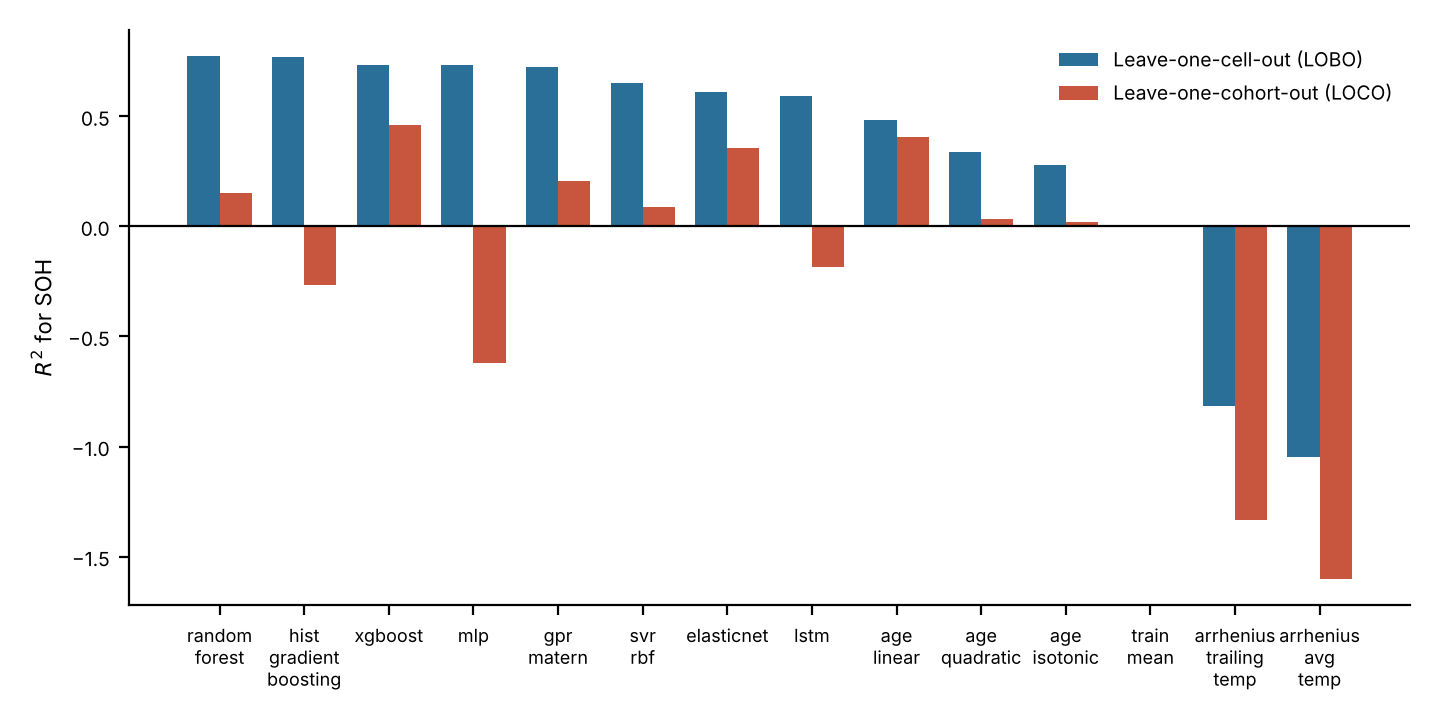
\includegraphics[width=\linewidth,height=0.35\textheight,keepaspectratio]{images/bench_lobo_loco.png}
    \caption{LOBO and LOCO $R^2$ for SOH for every scored method on the 31-cell NASA benchmark (data: \texttt{benchmark\_results.csv}). Skill measured across cells does not carry over to a new protocol.}
    \label{fig:benchbar}
\end{figure}


An ablation isolates where the skill comes from (Table~\ref{tab:ablation}). XGBoost on cycle number alone scored a LOCO $R^2$ of $-0.27$, and on behaviour features alone $-0.29$. Only their combination reached 0.459, while a straight line on cycle number reached 0.406. Shuffling each cell's capacity in time placed every LOCO interval at or below zero, so the harness does not manufacture skill. Usage features therefore added about 0.05 in $R^2$ over counting cycles, within the intervals.

\begin{table}[htbp]
	\caption{Feature Ablation and Shuffle Control (NASA SOH, LOCO)}
	\centering
	\small
	\renewcommand{\arraystretch}{1.15}
	\setlength{\tabcolsep}{4pt}
	\begin{tabular}{|L{0.38\linewidth}|L{0.17\linewidth}|C{0.12\linewidth}|C{0.2\linewidth}|}
		\hline
		\textbf{Run} & \textbf{Method} & \textbf{LOCO $R^2$} & \textbf{95\% CI} \\
		\hline
		All features (published) & XGBoost & 0.459 & [$-2.80$, 0.86] \\
		\hline
		All features (published) & Age-linear & 0.406 & [$-0.43$, 0.51] \\
		\hline
		Cycle number only & XGBoost & $-0.266$ & [$-1.15$, 0.82] \\
		\hline
		Behaviour features only & XGBoost & $-0.293$ & [$-0.72$, 0.80] \\
		\hline
		Shuffled in time (control) & Age-linear & $-0.039$ & [$-0.35$, $-0.004$] \\
		\hline
		Shuffled in time (control) & XGBoost & $-0.436$ & [$-1.44$, $-0.008$] \\
		\hline
	\end{tabular}
	\label{tab:ablation}
\end{table}

Temperature was the only usage factor with a consistent, correctly signed within-protocol relationship to fade (seven of seven cells in the two cohorts where it was significant), and its magnitude did not transfer between protocols. The rule-based risk score did not track measured fade either ($\rho = -0.27$, $p = 0.12$, on the 33 cells of the earlier health-index ranking), so it is labelled a heuristic.

\textbf{Interpretation.} No fitted method retains reliable skill under a change of protocol, and no method can be distinguished from another. This is the result that motivates the rest of the project: the estimators that ship fit nothing across cells.

\section{FIELD STATE-OF-HEALTH ESTIMATION}
\label{sec:res-field}

Table~\ref{tab:field} compares three ohmic treatments at the primary window on 22 CALCE cells. The field correction matched the laboratory correction within its interval and measured five more cells than no correction. Sensitivity windows gave 1.2\% (4.05--3.55~V, 16 cells) and 1.9\% (3.85--3.55~V, 17 cells).

\begin{table}[htbp]
	\caption{Field SOH at the 3.90--3.60~V Window; Median Per-Cell Absolute Error Against Cycler Capacity, 95\% Bootstrap Interval Over Cells}
	\centering
	\small
	\renewcommand{\arraystretch}{1.15}
	\setlength{\tabcolsep}{4pt}
	\begin{tabular}{|L{0.38\linewidth}|C{0.1\linewidth}|C{0.11\linewidth}|C{0.15\linewidth}|C{0.1\linewidth}|}
		\hline
		\textbf{Ohmic correction} & \textbf{Cells} & \textbf{Median} & \textbf{95\% CI} & \textbf{Worst} \\
		\hline
		None & 12/22 & 4.3\% & 2.5--5.4\% & 6.4\% \\
		\hline
		Cycler resistance (laboratory only) & 12/20 & 1.4\% & 1.2--2.5\% & 5.6\% \\
		\hline
		\textbf{Step resistance (field)} & \textbf{17/21} & \textbf{1.7\%} & \textbf{1.4--4.3\%} & \textbf{10.3\%} \\
		\hline
	\end{tabular}
	\label{tab:field}
\end{table}

The denominators differ because a correction can only be scored on cells for which it exists: one cell never rests before discharging, so no step resistance exists for it, which gives 17 of 21 cells for the field arm and 17 of 22 once that cell is counted as refused. The three worst cells (6.4--10.3\%) are all Type~3, whose discharge switches rate within a cycle. Every refusal carries a stated cause: four storage and partial-protocol cells delivered 80--155 equivalent full cycles before any constant-current discharge crossed the window, so the reference gate refused them, and one cell never rests before discharging. Fig.~\ref{fig:track} tracks the estimate against every laboratory capacity test, and Fig.~\ref{fig:cells} shows every measured cell.

\begin{figure}[htbp]
    \centering
    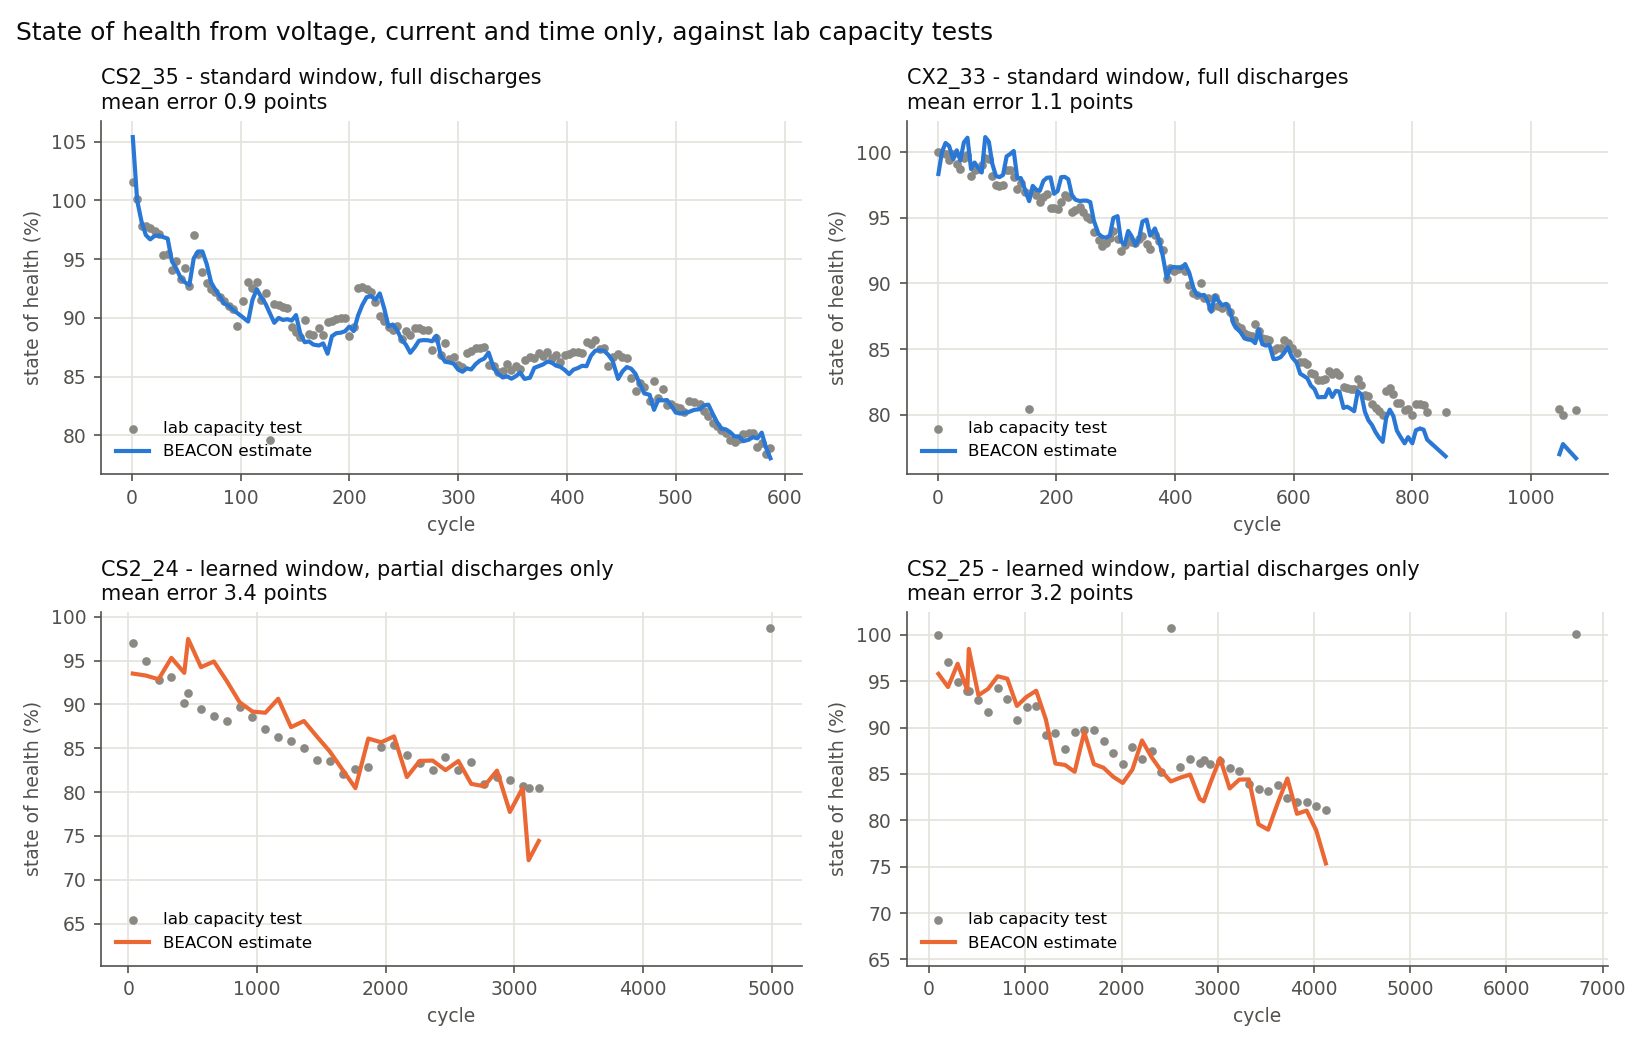
\includegraphics[width=\linewidth]{images/results_soh_tracking.png}
    \caption{SOH from voltage, current and time against every laboratory capacity test. Top: two constant-current cells, fixed window (mean error 0.9 and 1.1 points). Bottom: two cells of real partial cycling, learned window, estimate from partial discharges only (3.4 and 3.2 points).}
    \label{fig:track}
\end{figure}

\begin{figure}[htbp]
    \centering
    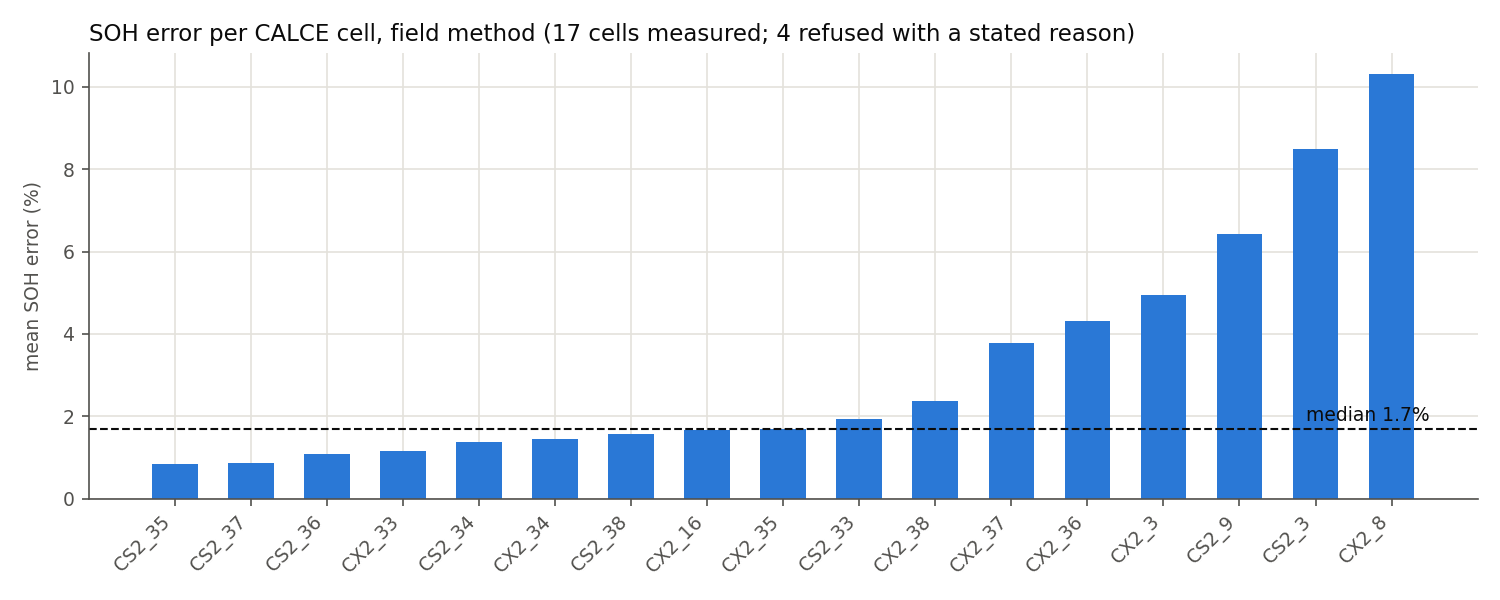
\includegraphics[width=\linewidth]{images/results_soh_per_cell.png}
    \caption{Mean absolute SOH error for every measured CALCE cell, field method; the dashed line is the median (1.7\%).}
    \label{fig:cells}
\end{figure}

\textbf{Interpretation.} Identifying resistance from the load step took the median error from 4.3\% to 1.7\% and the coverage from 12 to 17 cells, without any quantity the cycler computed. Two earlier figures were corrected downward by this work: an earlier SOH figure and an 88\% RUL figure had been scored against a reference capacity taken from each cell's whole life, which uses the future and which no BMS can hold.

\section{PARTIAL DISCHARGES}
\label{sec:res-partial}

On the four cells of real partial cycling (Table~\ref{tab:partial}), estimates use only the partial discharges preceding each laboratory check. Before the knee gate existed, the two near-empty cells were reported at 6.8\% and 12.8\% error while appearing confident. Learned windows on the 18 full-discharge cells have steepness 0.44--0.88, so any threshold between about 0.9 and 8 gives the same verdict on every cell and the chosen 2.0 is not tuned. As a control, the learned mode on those 18 cells measured 16 at a median of 1.95\%, beside 1.7\% for the fixed window, so it is a fallback and not a replacement.

\begin{table}[htbp]
	\caption{SOH from Real Partial Cycling (CALCE CS2 Types 5 and 6)}
	\centering
	\small
	\renewcommand{\arraystretch}{1.15}
	\setlength{\tabcolsep}{4pt}
	\begin{tabular}{|L{0.13\linewidth}|L{0.22\linewidth}|C{0.2\linewidth}|C{0.12\linewidth}|L{0.17\linewidth}|}
		\hline
		\textbf{Cell} & \textbf{Band} & \textbf{Learned window} & \textbf{Steepness} & \textbf{Result} \\
		\hline
		CS2\_24 & top of charge & 4.00--3.82~V & 0.83 & 3.4\% error \\
		\hline
		CS2\_25 & top of charge & 4.03--3.83~V & 0.82 & 3.2\% error \\
		\hline
		CS2\_5 & near empty & -- & 10.4 & refused (knee) \\
		\hline
		CS2\_6 & near empty & -- & 8.2 & refused (knee) \\
		\hline
	\end{tabular}
	\label{tab:partial}
\end{table}

\textbf{Interpretation.} The refusal is physics and not a tuned cut. On the plateau, window charge tracks capacity, while on the knee voltage is set by resistance and diffusion, so it measures how hard the cell is working instead. The scope is two cells per band, which shows the mechanism and is too few to quote a population error.

\section{INTERNAL RESISTANCE ESTIMATION}
\label{sec:res-r}

Against the cycler's internal-resistance column over each cell's life (20 cells carrying both values), the step resistance achieved a median Spearman correlation of 0.86, growth in the same direction on 19 of 20 cells, and a median growth of 1.26 times against the cycler's 1.29 times. This includes the partial-cycling cells (0.90 and 0.98), and the exception is a Type~3 cell. The levels differ, since the step value includes early polarisation, but the trends agree, which is what a power-fade indicator requires.

\section{REMAINING USEFUL LIFE}
\label{sec:res-rul}

At threshold 0.90, referenced to each cell's first cycles (17 cells), Table~\ref{tab:rul} reports accuracy by the true distance to end of life and by the prediction a user sees. Near end of life the estimate is a safe lower bound: it warns early and almost never late. Errors are predominantly early because these cells fade quickly at first and then more slowly, so a full-history line is steeper than the remaining fade.

\begin{table}[htbp]
	\caption{RUL to 90\% Capacity. Left: By True Cycles to End of Life. Right: By Predicted Cycles, With the 90\% Range of (True $-$ Predicted)}
	\centering
	\footnotesize
	\renewcommand{\arraystretch}{1.15}
	\setlength{\tabcolsep}{3pt}
	\begin{tabular}{|C{0.1\linewidth}|C{0.11\linewidth}|C{0.1\linewidth}|C{0.11\linewidth}|C{0.14\linewidth}|C{0.15\linewidth}|}
		\hline
		\textbf{True} & \textbf{Within $\pm$20} & \textbf{Median err.} & \textbf{Predicted} & \textbf{Lasted $\ge$ pred.} & \textbf{90\% range} \\
		\hline
		0--25 & 73\% & 9.6 & 0--25 & 95\% & $+1$ to $+82$ \\
		\hline
		25--50 & 44\% & 22.8 & 25--50 & 88\% & $-14$ to $+129$ \\
		\hline
		50--100 & 15\% & 42.7 & 50--100 & 85\% & $-40$ to $+141$ \\
		\hline
		200--400 & 0\% & 144 & -- & -- & -- \\
		\hline
	\end{tabular}
	\label{tab:rul}
\end{table}

Scored against a reference capacity taken as the 95th percentile of the cell's whole record, the same estimator was within $\pm$20 cycles 88\% of the time near end of life. That reference uses the future, which no BMS can hold. Against the cell's own early capacity the figure is 73\%, and that is the figure reported. Fig.~\ref{fig:rul} summarises the result.

\begin{figure}[htbp]
    \centering
    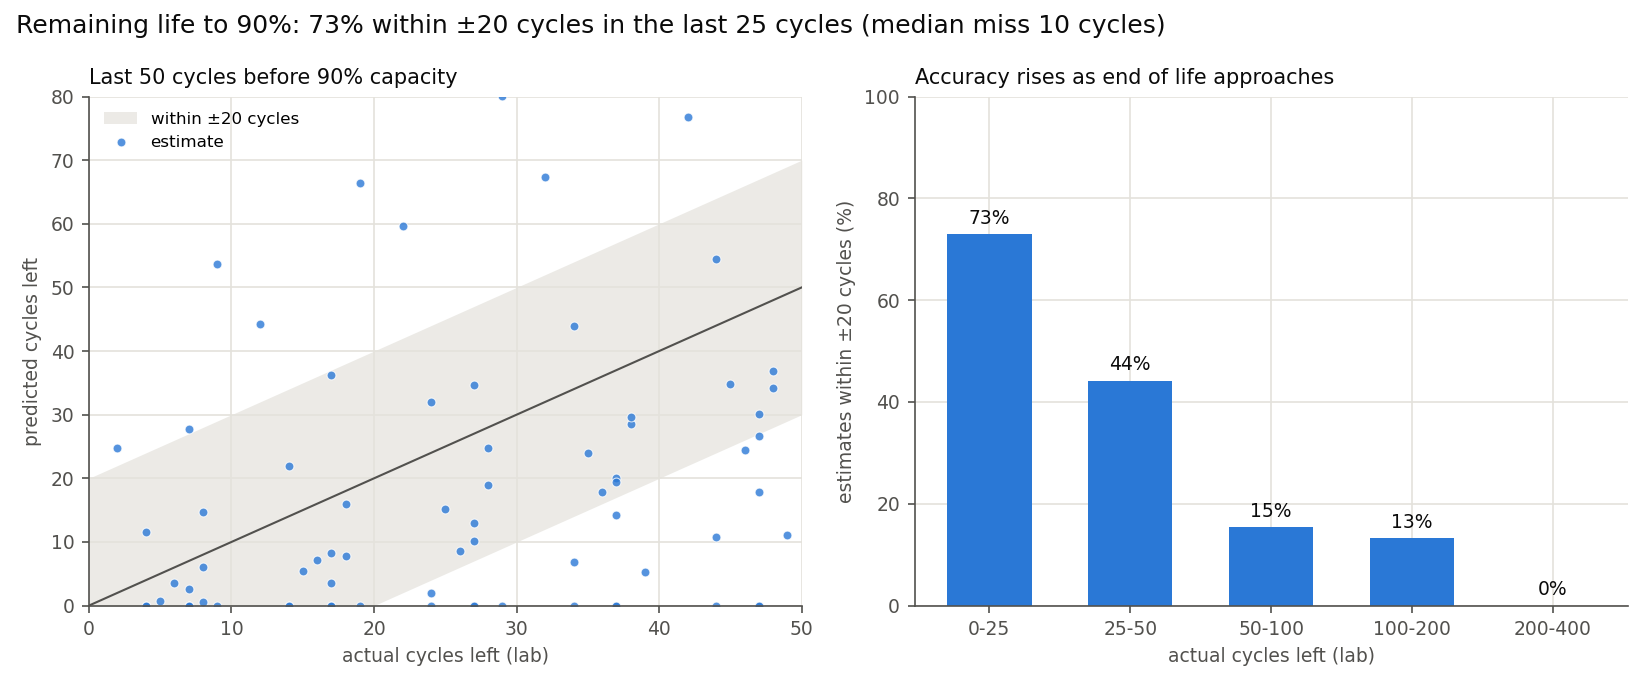
\includegraphics[width=\linewidth]{images/results_rul.png}
    \caption{RUL to 90\% capacity. Left: predicted against actual cycles left in the last 50 cycles. Right: share of estimates within $\pm$20 cycles by actual distance to end of life.}
    \label{fig:rul}
\end{figure}

\textbf{Interpretation.} The ``within $\pm$20 cycles'' claim is true near end of life and false far from it (0\% at 200 or more cycles out), so it is reported with its condition and not bare. The conservative direction is a property of the 90\% threshold on these cells and is not a general guarantee. At an 85\% threshold the median bias near end of life turns positive (+6.7 cycles within 25 cycles of end of life), so the estimate runs late there and only 62.8\% of estimates fall within $\pm$20 cycles. The conventional 80\% end-of-life threshold is not validated on CALCE, because its full-discharge trajectories end near 0.81 and only one cell of 22 crosses 0.80.

\section{RUL ESTIMATION UNDER SPARSE COMPLETE DISCHARGES}
\label{sec:res-sparse}

A driver who seldom fully discharges produces few complete discharges (on the partial-cycling cell CS2\_24 they are rare). Four methods were evaluated on the same sparse evidence (Table~\ref{tab:sparse}). Sparsity is real on the partial-cycling cells and emulated as one complete discharge in 50 on the constant-current cells.

\begin{table}[htbp]
	\caption{RUL from Sparse Complete Discharges; None Is Accurate Enough to Report}
	\centering
	\small
	\renewcommand{\arraystretch}{1.15}
	\setlength{\tabcolsep}{4pt}
	\begin{tabular}{|L{0.4\linewidth}|L{0.46\linewidth}|}
		\hline
		\textbf{Method} & \textbf{Outcome} \\
		\hline
		Sparse capacity, standard minimum & Refuses every point (never reaches 30) \\
		\hline
		Field SOH trajectory & Answers 62\%; median miss 79 cycles when predicting under 25 \\
		\hline
		Field SOH scaled by the cell's own complete discharges & Over-corrects; errors turn late near end of life \\
		\hline
		Sparse capacity, minimum lowered to 5 (post hoc) & 0\% within $\pm$20 cycles; misses late \\
		\hline
	\end{tabular}
	\label{tab:sparse}
\end{table}

The failure of the field-trajectory method has a clean cause. Near 0.90, field SOH reads a median 1.1 points below capacity (measured in a first pass of this study, not kept as a separate artifact). Because fade near the threshold is slow, that small bias moves the 0.90 crossing a median 56 cycles early. An SOH error that is acceptable as a health figure thus becomes large as a time to threshold. None of the four is reported, and the system refuses RUL for partial-only records and states that this was tested.

\section{EVIDENCE SUFFICIENCY ANALYSIS}
\label{sec:res-suff}

Three questions were fixed before the study and scored at every laboratory check on 19 cells. First, \emph{count does not predict accuracy}: median error was 0.75\% at 6--10 usable readings and 1.97\% beyond 60, because error grows with age as the approximation in Eq.~\eqref{eq:soh} drifts. A rule of high confidence after a fixed number of discharges therefore has no support. Second, \emph{consistency does} (Table~\ref{tab:suff}). The pooled Spearman correlation between $u$ and absolute error was 0.48. Within cells it was weaker (median 0.14, positive in 14 of 19), so $u$ chiefly separates unreliable cells and periods and does not rank readings within a good one.

\begin{table}[htbp]
	\caption{Error by the Consistency Criterion of Eq.~\eqref{eq:u}}
	\centering
	\small
	\renewcommand{\arraystretch}{1.15}
	\setlength{\tabcolsep}{4pt}
	\begin{tabular}{|L{0.34\linewidth}|C{0.12\linewidth}|C{0.1\linewidth}|C{0.13\linewidth}|C{0.14\linewidth}|}
		\hline
		\textbf{Readings} & \textbf{Points} & \textbf{Cells} & \textbf{Median error} & \textbf{90th percentile} \\
		\hline
		$u \le 0.01$ (consistent) & 8,993 & 16 & 1.3\% & 4.4\% \\
		\hline
		$u > 0.01$ (inconsistent) & 2,168 & 13 & 5.1\% & 21.9\% \\
		\hline
	\end{tabular}
	\label{tab:suff}
\end{table}

Third, \emph{reference size}: in the study's own scoring, larger references reduced error (one discharge 3.6\%, five 2.0\%, ten 1.3\%), but on the field-study metric ten versus five changed the median only from 1.681\% to 1.665\%, so the estimator retains five.

\section{EXTERNAL VALIDATION ON A SECOND DATASET}
\label{sec:res-oxford}

The estimator was applied to the eight Oxford cells without re-tuning. Arms, reference and scoring were fixed before the run. The reference is each cell's first characterisation, and truth is 1C capacity relative to it. Because each characterisation block begins under load, no rest-to-load step exists, so the 1C window is uncorrected.

\begin{table}[htbp]
	\caption{External Validation on Eight Oxford Cells: Median and Worst Per-Cell Mean Absolute SOH Error}
	\centering
	\small
	\renewcommand{\arraystretch}{1.15}
	\setlength{\tabcolsep}{4pt}
	\begin{tabular}{|L{0.5\linewidth}|C{0.1\linewidth}|C{0.12\linewidth}|C{0.1\linewidth}|}
		\hline
		\textbf{Window} & \textbf{Cells} & \textbf{Median} & \textbf{Worst} \\
		\hline
		Fixed 3.90--3.60~V, 1C discharge & 8/8 & 3.0\% & 4.0\% \\
		\hline
		Fixed 3.90--3.60~V, C/18 pseudo-OCV & 8/8 & 3.2\% & 3.4\% \\
		\hline
		Learned window, 1C discharge & 8/8 & 2.3\% & 3.6\% \\
		\hline
	\end{tabular}
	\label{tab:oxford}
\end{table}

All eight cells were measured (Table~\ref{tab:oxford}). The near-equilibrium C/18 window was not more accurate than the 1C window, so on this blend cathode the residual error stems from the curve changing shape with age and not from ohmic sag, consistent with the stated approximation of Eq.~\eqref{eq:soh}.

\paragraph{Drive-Cycle Discharge.} The drive-cycle discharge of Cell~1 has current between $-5.0$ and $+1.6$~A. Resistance from its own 1,575 current steps of at least 0.2~A gave a median of 21~m$\Omega$ (interquartile 19--24). The discharge is itself partial (it stops at about 65\% depth), so a coverage window (4.08--3.78~V) was chosen from the corrected curve's span alone, before any comparison was computed. In it the drive-cycle reading, corrected per sample and fitted monotonically, was 0.2625~Ah, against 0.2661~Ah from the same cell's 1C constant-current discharge, a difference of 1.4\%. Both lay about 13\% below the C/18 reading in that window, so the rate effect cancels in a ratio of like with like but would bias one that mixed rates. This is a single discharge and demonstrates the mechanism, not a population error.

\paragraph{Remaining Life at the 80\% Threshold.} The Oxford trajectories cross the 80\% convention, so the shipped RUL estimator was scored there unchanged. When it predicted fewer than 500 cycles to 80\%, the cell lasted at least that long in 97\% of cases (36 estimates, 5 cells). Precision is low: the median miss is 385 cycles against characterisations 100 cycles apart. The guarantee also weakens with distance, since predictions of 500 to 1,000 cycles were met or exceeded only 80\% of the time (25 estimates, 5 cells).

\section{VALIDATION ON A THIRD DATASET AND REFUSAL BEHAVIOUR}
\label{sec:res-xds}

The NASA files (18650 cells, ambient 4--44~$^\circ$C) were read from their original MATLAB form and scored the same way, unchanged. The estimator was poor on NASA overall, with a median per-cell error of 9.2\% over 27 cells, and it depended on temperature: 1.7\% in the 43~$^\circ$C cohort and 12--14\% at 4 and 22~$^\circ$C. The step resistance captures only the ohmic part of the overpotential, and at low temperature the charge-transfer and diffusion parts, which grow with age, move the curve through the window.

The consistency uncertainty, with its tolerance fixed on CALCE, was applied unchanged. On NASA, estimates it labelled HIGH or MEDIUM had a median per-cell error of 4.5\%, while those labelled LOW had 13.2\% (within three SOH points: 49\% versus 12\%). The failure on unseen conditions was thus largely signalled by the estimator itself.

For contrast, a gradient-boosted model on three window features, the setting where fitting looks best, reached 0.7\% under leave-one-cell-out within Oxford and 1.2\% within CALCE, but 6.7\% when moved from Oxford to NASA and 5.5\% from CALCE to Oxford. Validation inside one dataset overstated transferable accuracy four- to tenfold.

\section{SYSTEM AND HARDWARE RESULTS}
\label{sec:res-system}

\subsection{Bench Rig Captures}

Three captures are discussed here (Table~\ref{tab:captures}); the repository holds further bring-up files, including one garbled capture from the baud-rate fault and one longer synthetic run. The first is a counter-example: a board with no sensors attached, whose synthetic profile still scores, and which is kept and labelled as such.

\begin{table}[htbp]
	\caption{Bench Rig Captures}
	\centering
	\footnotesize
	\renewcommand{\arraystretch}{1.15}
	\setlength{\tabcolsep}{3pt}
	\begin{tabular}{|L{0.22\linewidth}|L{0.2\linewidth}|C{0.12\linewidth}|L{0.22\linewidth}|}
		\hline
		\textbf{Capture} & \textbf{Declared channels} & \textbf{Records} & \textbf{Measured} \\
		\hline
		Stage A (no sensors) & all, from stubs & 151 & Synthetic, not a hardware result \\
		\hline
		Stage B voltage & $t$, $v$, $i$, SOC (INA219 up, LM35 refused) & 83 over 82~s & 3.9871~V (sd 1.9~mV); current at the $\pm$0.4~mA noise floor \\
		\hline
		Temperature demo & $t$, $t_c$ (LM35 up, INA219 refused) & 85 over 84~s & 32.11~$^\circ$C (sd 0.086~$^\circ$C) \\
		\hline
	\end{tabular}
	\label{tab:captures}
\end{table}

In both real captures the cadence held at 1.000~s with no gaps and a monotonic time base. Every measured voltage is an exact multiple of the INA219's 4~mV bus LSB, which is what a genuine read from that part looks like and what a fabricated one would not. The sensor-complement declaration worked as designed: the firmware named the sensor that failed at boot, declared only the channels it could supply, and the host scored those and refused the rest by name. The first real board also exposed a baud-rate fault (the CH340 bridge accepts only 9600 and 19200 baud), which the refusal wording named as a cause and which led to the fix.

Fig.~\ref{fig:rigcapture} plots the Stage B capture and Fig.~\ref{fig:uievidence} shows how the dashboard presents it.

\begin{figure}[htbp]
    \centering
    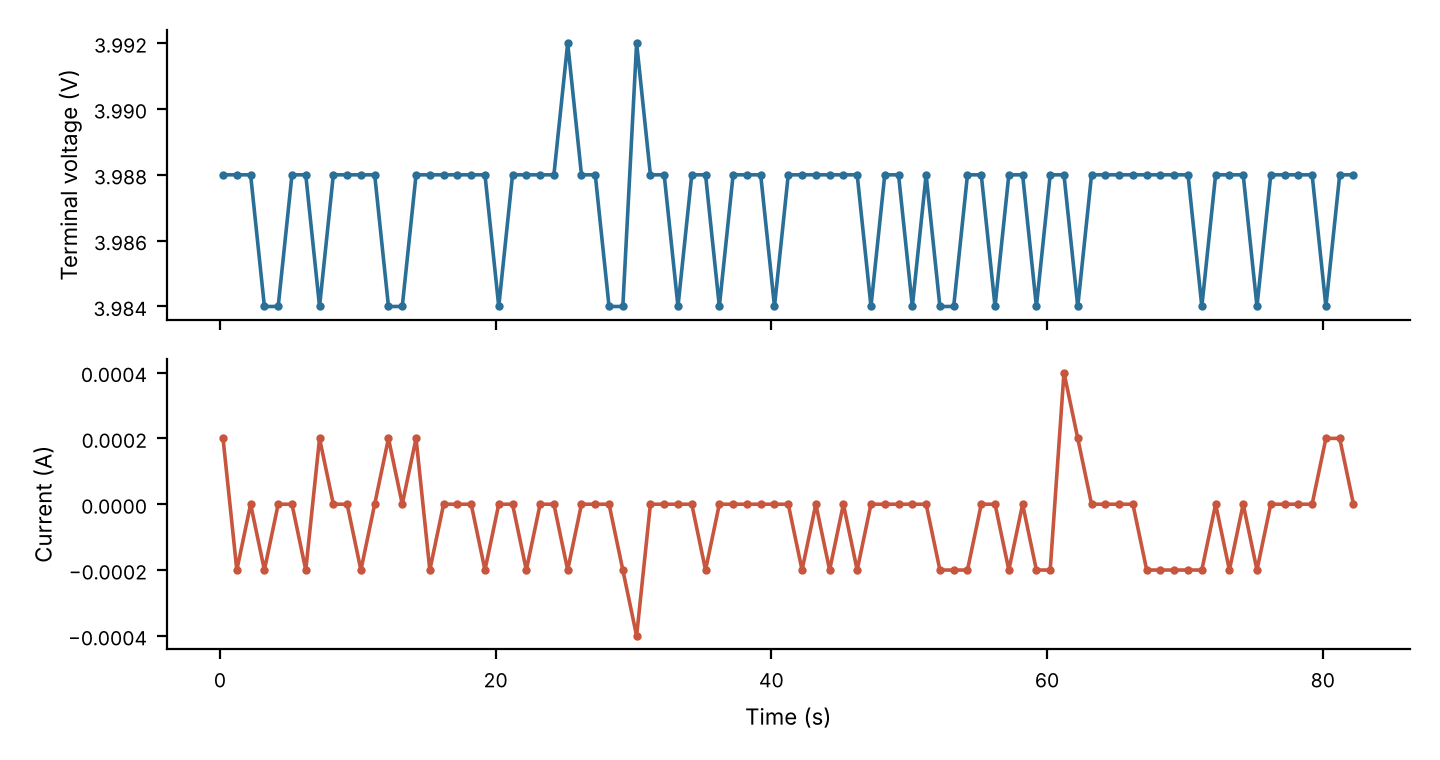
\includegraphics[width=\linewidth,height=0.35\textheight,keepaspectratio]{images/rig_capture.png}
    \caption{Stage B capture from the bench rig (83 frames over 82~s, one cell at rest). Voltage moves between 3.984 and 3.992~V in steps of the INA219's 4~mV LSB, and current stays at the $\pm$0.4~mA noise floor.}
    \label{fig:rigcapture}
\end{figure}

\begin{figure}[htbp]
    \centering
    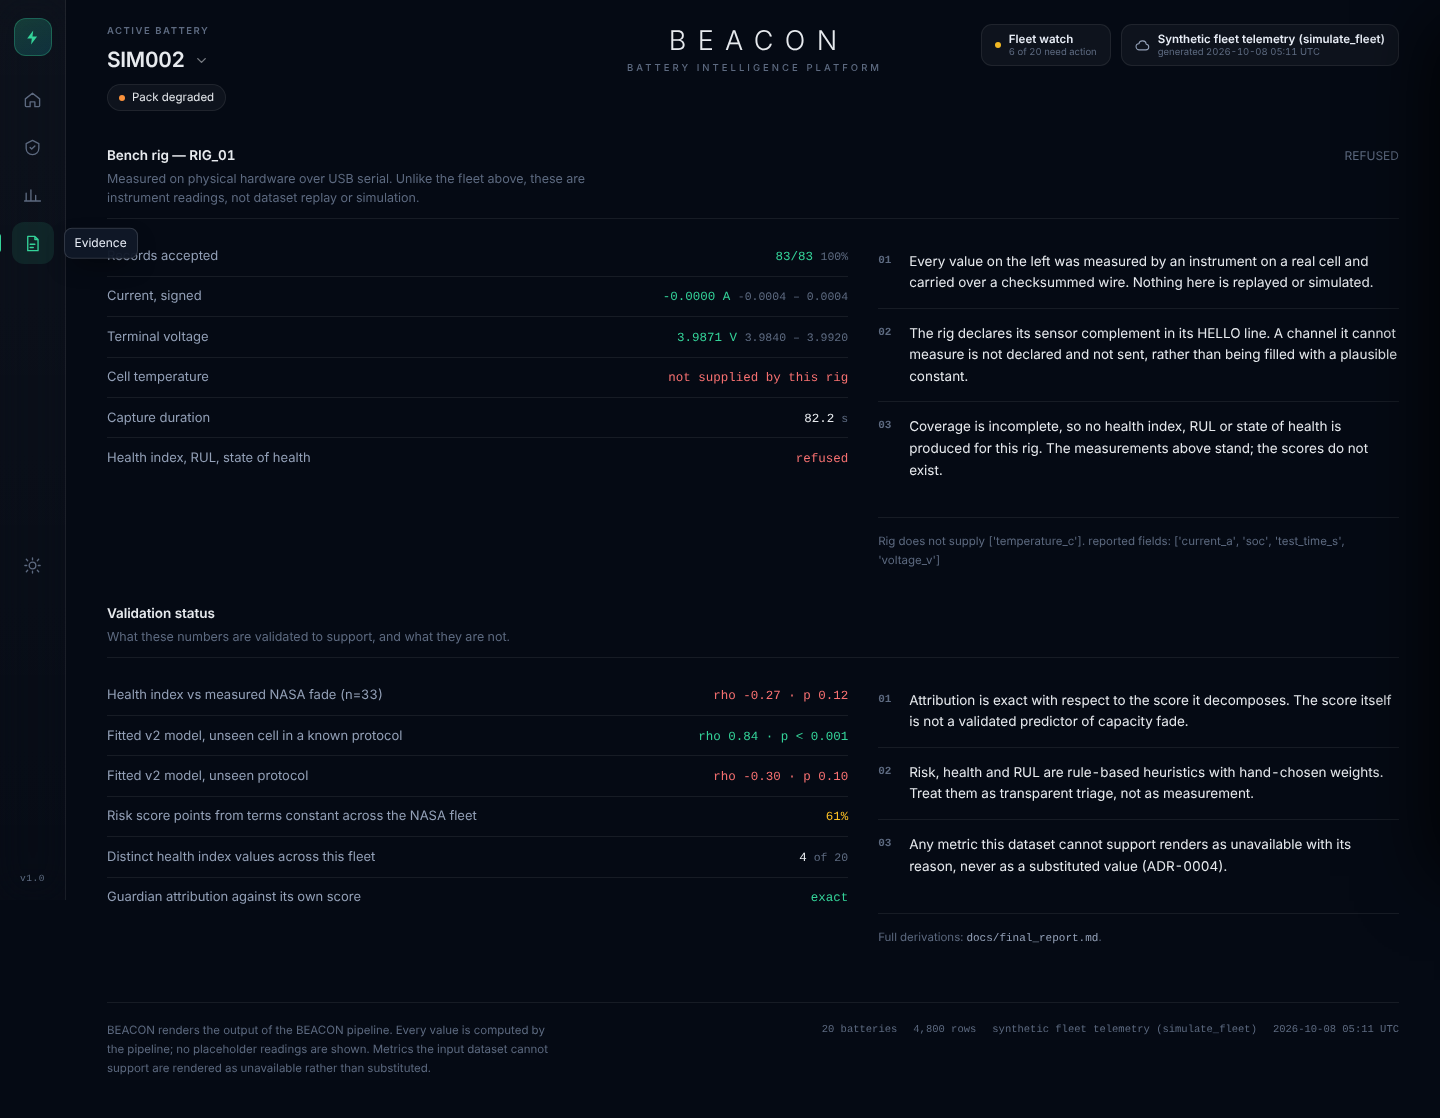
\includegraphics[width=\linewidth,height=0.45\textheight,keepaspectratio]{images/ui_evidence.png}
    \caption{Evidence view of the BEACON dashboard for the bench rig: 83 of 83 records accepted, voltage and current as measured, temperature reported as not supplied, and the health index, remaining life and state of health refused because coverage is incomplete.}
    \label{fig:uievidence}
\end{figure}


\subsection{Fault Injection}

Faults injected into a real capture behaved as designed: a corrupted byte failed its checksum, a NaN field was rejected, a reversed timestamp refused the capture, and a missing sensor was refused by name. The injection also exposed one defect, since corrected: a 999~V reading passed the field range, which is wide so that packs are admissible. Records outside 0--5~V are now rejected when the source declares a single cell.

\subsection{What the Hardware Result Does and Does Not Show}

The captures demonstrate that the transport, the protocol, the gate and the refusal path work against real silicon. They are one cell, at rest, for under 90~s, with no load step and no charge or discharge cycle. They are \emph{not} a validation of the health, RUL or risk models, which were fitted on cycled research cells and cannot be confirmed or refuted by a cell that was never cycled. Sensor accuracy against a reference meter was not measured, and no discharge has yet been recorded on the rig.

\section{ILLUSTRATIVE EXAMPLE: THE HEALTH REPORT CARD}
\label{sec:res-card}

Fig.~\ref{fig:card} abridges the report card for CALCE cell CS2\_35 as it would have read at cycle 90. The pipeline saw voltage, current and time only.

\begin{figure}[htbp]
    \centering
    {\footnotesize
\begin{verbatim}
1. HOW HEALTHY IT IS
   91.0% state of health  [MEASURED]   State: WARNING
2. HOW LONG IT HAS LEFT
   About 5 cycles until it falls to 90% of its early
   capacity.  [ESTIMATE]
3. WHAT YOUR USAGE IS DOING TO IT
   No temperature was measured, so heat exposure cannot
   be assessed.
4. WHAT TO DO
   Capacity fade is measurable. Keep monitoring.
5. WHAT THIS REPORT CANNOT TELL YOU
   - Scoring skipped: required channels not supplied.

CHECK AGAINST THE LAB (the card was not shown this)
   Lab capacity at cycle 90: 91.4%; card said 91.0%
   Cell actually crossed 90% at cycle 146: 56 cycles
   after cycle 90; card said 5
\end{verbatim}}
    \caption{Abridged health report card for CS2\_35 at cycle 90, with the laboratory check.}
    \label{fig:card}
\end{figure}

The health figure is within half a point. The remaining-life figure is 51 cycles early, which is the conservative bias the RUL study measured at that distance (median $-32$ cycles at 50--100 cycles out), and it is the reason the card prints its own accuracy beside the number and not the number alone. Only temperature is offered as a usage finding, because it is the one behaviour-to-ageing link that survived testing, in direction only.

\section{DISCUSSION}
\label{sec:discussion}

\paragraph{Effect of Conditioning Versus Model Choice.} Across fourteen scored methods, LOCO differences were smaller than the uncertainty on any one of them. Three conditioning decisions, by contrast, changed error by multiples. Refusing truncated discharges took the worst cell from 52\% to about 10\%. Identifying resistance from the load step took the median from 4.3\% to 1.7\% and coverage from 12 to 17 cells. Refusing knee windows converted 6.8--12.8\% errors into refusals. For a BMS software layer, the leverage lies in what is measured and how it is conditioned, not in the regressor that follows. The first of these was a misdiagnosis corrected during the project: the 52\% worst case had been attributed to loss of active material, when it was actually truncated discharges being read as full ones.

\paragraph{Dependence on the Reference Definition.} Two results moved when the reference was made one a BMS can hold: RUL accuracy fell from 88\% to 73\%, and a partial-discharge reference formed from a late discharge produced a large error until the timing gate existed. Validation should use the reference the deployed system will have.

\paragraph{Sensitivity of Threshold Crossings to Bias.} A 1.1-point SOH bias, unremarkable as a health figure, shifted predicted end of life by about 56 cycles. Any RUL built on an estimated rather than measured SOH inherits this, and should be evaluated as a time to threshold and not through SOH error.

\paragraph{Quantifying Evidence Sufficiency.} Treating ``enough data'' as a count is intuitive and here wrong, because the estimator's error is dominated by age-related drift and not sampling. The consistency of readings is observable without ground truth and separates 1.3\% from 5.1\% median error, which gives a BMS layer a principled way to report ``not yet'' for a battery it has never seen.

\paragraph{Limitations of the Findings.}
\begin{itemize}
    \item \emph{Temperature.} On NASA cells at 4 and 22~$^\circ$C the estimator erred by 12--14\%. The low-confidence label marked most of these readings, but a temperature-aware correction is future work.
    \item \emph{Two cathode families, single cells, one real drive cycle.} Packs add cell-to-cell imbalance, thermal gradients and balancing currents, and the flat plateau of lithium iron phosphate would challenge the window method directly.
    \item \emph{Two cells per partial-cycling band.}
    \item \emph{End of life:} validated at 90\% on CALCE, and at 80\% on Oxford only as a conservative bound with low precision.
    \item \emph{Apparent resistance} depends on the logger's sample interval and is comparable within a record, not across loggers.
    \item \emph{No hardware discharge} has yet been recorded on the bench rig, and the heuristic risk layer is not validated.
\end{itemize}

\section{IMPLICATIONS FOR BMS SOFTWARE DESIGN}

Four implications follow from the results and are stated here as design guidance for a software layer above a BMS.

\paragraph{Validate on the Unit of Deployment.} A model is deployed on a battery that has not been seen and often on a protocol that has not been seen. The validation split should hold out that unit, and the interval around the result should be reported, because on the benchmark of this project the interval on a single method was wider than the difference between methods.

\paragraph{Prefer Measurement to Fitting Where Measurement Is Possible.} Voltage, current and time are enough to measure capacity on a discharge that spans a voltage window, and the measurement needs no training cells. Fitting is then needed only for the quantities that cannot be measured directly.

\paragraph{Make Refusal a Normal Output.} A refusal that carries its cause is information, since it tells the operator what data to collect. The consistency criterion separated a 4.5\% median error from a 13.2\% median error without any knowledge of the true capacity, which shows that a system can recognise its own poor conditions.

\paragraph{Keep One Scoring Path.} When a vehicle, a rig and a dataset all pass through the same function, a result obtained on a dataset says something about the vehicle, and a defect found on the rig is fixed for all three.

\section{VALIDATION SUMMARY}

Table~\ref{tab:summary} lists the outputs by status. Claims that failed or were never tested are listed, because that is what makes the others believable.

\begin{table}[htbp]
	\caption{Status of the Main Outputs}
	\centering
	\footnotesize
	\renewcommand{\arraystretch}{1.15}
	\setlength{\tabcolsep}{3pt}
	\begin{tabular}{|L{0.34\linewidth}|L{0.34\linewidth}|L{0.2\linewidth}|}
		\hline
		\textbf{Output} & \textbf{Result} & \textbf{Status} \\
		\hline
		Capacity health (full discharges) & 1.7\% median, 17 of 22 cells & Validated \\
		\hline
		Capacity health (partial discharges) & 3.2--3.4\%, 2 cells & Validated, 2 cells \\
		\hline
		Resistance health & Same direction on 19 of 20 cells & Validated \\
		\hline
		RUL near end of life & 73\% within $\pm$20 cycles & Validated, 90\% threshold \\
		\hline
		RUL far from end of life & 0\% at 200--400 cycles & Not valid (shown with band) \\
		\hline
		RUL from sparse complete discharges & Four methods, none accurate & Refused \\
		\hline
		Second dataset (Oxford) & 3.0\% median, 8 of 8 cells & Validated \\
		\hline
		Third dataset (NASA) & 9.2\% overall, 1.7\% at 43~$^\circ$C & Fails outside warm conditions \\
		\hline
		Fitted models across protocols & Best LOCO $R^2$ 0.459, CI [$-2.80$, 0.86] & Not generalising \\
		\hline
		Heuristic risk score & $\rho=-0.27$, $p=0.12$ & Labelled heuristic \\
		\hline
		Telemetry on hardware & 83/83 frames, 1.000~s cadence & Validated (acquisition only) \\
		\hline
		Health from a real rig discharge & No discharge recorded & Not tested \\
		\hline
		Packs, LFP, large-scale drive cycles & No data & Not tested \\
		\hline
	\end{tabular}
	\label{tab:summary}
\end{table}

\section{ASSESSMENT AGAINST THE OBJECTIVES}

Table~\ref{tab:objectives} relates each objective of Section~1.5 to the evidence for it in this chapter and in Chapter~\ref{ch:implementation}.

\begin{table}[htbp]
	\caption{Objectives and Evidence}
	\centering
	\footnotesize
	\renewcommand{\arraystretch}{1.1}
	\setlength{\tabcolsep}{3pt}
	\begin{tabular}{|C{0.05\linewidth}|L{0.42\linewidth}|L{0.34\linewidth}|}
		\hline
		\textbf{No.} & \textbf{Objective} & \textbf{Evidence} \\
		\hline
		1 & End-to-end ingestion of CAN, serial and dataset sources through one pipeline & Single scoring function; three transports; test modules and continuous integration \\
		\hline
		2 & SOH from voltage, current and time with ohmic correction & 1.7\% median error on 17 of 22 CALCE cells \\
		\hline
		3 & Resistance as a second quantity; RUL from each cell's own fade & Resistance trend in the same direction on 19 of 20 cells; 73\% of RUL within $\pm$20 cycles near end of life \\
		\hline
		4 & Measured evidence sufficiency; refusal of insufficient evidence & Consistency criterion separates 4.5\% from 13.2\% error; every refusal carries a reason \\
		\hline
		5 & External validation without re-tuning; retention of negative results & Oxford median error 3.0\%; sparse-discharge RUL and fitted-model ranking retained as negative results \\
		\hline
		6 & Physical rig, API and dashboard & 83 of 83 frames received; routes and dashboard served from containers \\
		\hline
	\end{tabular}
	\label{tab:objectives}
\end{table}

\section{THREATS TO VALIDITY}

The results are bounded by the way they were obtained, and the bounds are stated here so that they can be weighed against the figures.

\begin{itemize}
	\item \textbf{Chemistry and format.} Development and primary validation use LCO prismatic cells at constant current. The external dataset is an NMC/LCO blend pouch cell at one temperature. Results for lithium iron phosphate, for packs and for dynamic loads are not claimed.
	\item \textbf{Reference definition.} Two results moved when the reference was changed to the capacity the cell's own first discharges measure, which is what a BMS can know. A figure is therefore tied to the reference named with it.
	\item \textbf{Small numbers of cells.} Several results rest on a few cells, for example the partial-discharge result on two cells. They are reported as validated on those cells, and no claim is made beyond them.
	\item \textbf{Hardware.} The rig validates the data-acquisition path. No discharge has been recorded on it, so no health figure from the rig is claimed.
	\item \textbf{Heuristic layer.} The behaviour risk score was not significantly related to measured fade ($\rho=-0.27$, $p=0.12$ on the 33 cells of the earlier health-index ranking of the project, a slightly larger set than the 31-cell benchmark) and is labelled a heuristic wherever it appears.
\end{itemize}

\section{ROBUSTNESS AND SECURITY CHECKS}

Beyond estimation accuracy, the system was checked for the behaviour of its interfaces under bad input. The serial parser ignores lines without the sentinel as noise, counts and discards malformed lines, rejects out-of-range, non-finite and checksum-failed values instead of clamping them, and refuses a capture whose accepted fraction falls below a configured threshold. These behaviours are exercised by tests with truncated lines, corrupted checksums, non-finite values, out-of-range fields and unknown record types. The path-containment fix was verified by thirteen tests, and a search of the source files for keys, secrets and language-model clients found none, apart from a benign file name in a test. Continuous integration runs with no key, no hardware and no external service beyond the package registries, so the checks run the same way on every commit.

